%\VignetteIndexEntry{An introduction to the package geoRglm}
%\VignetteDepends{}
%\VignetteKeywords{spatial}
%\VignettePackage{geoRglm}
\documentclass[12pt,a4paper]{article}
\usepackage[latin1]{inputenc}
\usepackage[dvips]{graphicx}
%\usepackage{psfig,epsfig,psfrag}
\usepackage{color,enumerate,longtable}
\usepackage{texnames,lastpage,verbatim,fancyvrb}
%% possible conflicts with Rd.sty
%\usepackage{url,html}
%\usepackage{heqn}
%\usepackage{amssymb,amsmath,amsfonts}
%
% Page size
%
%\usepackage{setspace,calc}
%\setlength{\voffset}{-1.5in}
%\setlength{\hoffset}{-1in}
%\setlength{\topmargin}{30mm}
%\setlength{\oddsidemargin}{40mm}
%\setlength{\textwidth}{210mm-10mm-\oddsidemargin}
%\setlength{\textheight}{297mm-10mm-\topmargin-\headheight-\headsep}
%
% Sweave settings
%
% Setting default size for \includegraphics 
% setting global defaults for figures: directory, names and sizes  
%%%%% \ SweaveOpts{prefix.string=figures/fig,width=4,height=4}

% emulating Sweave: Sweave style for R input code and output
\DefineVerbatimEnvironment{Rin}{Verbatim}{fontshape=sl}
\DefineVerbatimEnvironment{Rout}{Verbatim}{}
\newcommand{\Rcmd}[1]{\textsl{\texttt{#1}}}

% loading Defs from Rd.sty
%% [OFC: few changes coz of local pdflatex font problems]
%\newcommand{\strong}[1]{{\normalfont\fontseries{b}\selectfont #1}}
\newcommand{\strong}[1]{{\textbf{ #1}}}
\let\pkg=\strong
\newcommand{\code}[1]{\texttt{\small #1}}
%\newcommand{\R}{{\normalfont\textsf{R}}{}}
\newcommand{\R}{{\textsf{R}}{}}
\newcommand{\sQuote}[1]{`#1'}
\newcommand{\dQuote}[1]{``#1''}
\let\command=\code

\title{\pkg{geoRglm} : a package for  generalised linear spatial models
\\{\it introductory session}}
\author{Ole F. Christensen \& Paulo J. Ribeiro Jr.}
\date{Last update: \today}

\usepackage{/users/olefc/local.1.9/lib/R/share/texmf/Sweave}
\begin{document}

\maketitle

%% Sweave settings for includegraphics default plot size (Sweave dafault is 0.8)  
%% notice this must be after begin{document}
%%% \setkeys{Gin}{width=0.9\textwidth}



The objective of this page is to introduce the reader to the 
\pkg{geoRglm} commands and show how they can be used.
The commands used here are basic examples of the package handling, where we typically use default arguments for the function calls.
We encourage the user also to inspect other function arguments.

For further details on the functions included in \pkg{geoRglm}, we refer to the \pkg{geoRglm} documentation.

\section{STARTING A SESSION AND LOADING DATA}
After starting an \R{} session, we first load \pkg{geoR} and \pkg{geoRglm} with the commands:
\begin{Schunk}
\begin{Sinput}
> library(geoR)
> library(geoRglm)
\end{Sinput}
\end{Schunk}

If the installation directories for the packages are not the default locations for \R{} packages, type:
\begin{Rin}
  library(geoR, lib.loc = "PATH_TO_geoR")
  library(geoRglm, lib.loc = "PATH_TO_geoRglm")
\end{Rin}
where \verb+PATH_TO_geoR+ and \verb+PATH_TO_geoRglm+ are the paths to the directories where \pkg{geoR} and \pkg{geoRglm} are installed, respectively.
If \pkg{geoRglm} is correctly loaded the following message will be displayed:
\begin{Schunk}
\begin{Soutput}
-----------------------------------------------------------
geoRglm - a package for generalised linear spatial models
geoRglm version 0.8-1 (2004-08-07) is now loaded
-----------------------------------------------------------
\end{Soutput}
\end{Schunk}
Helpfiles are available for \pkg{geoRglm}. For getting help on the function \code{glsm.mcmc}, just type:  
\begin{Rin}
> help(glsm.mcmc)
\end{Rin}


\section{DATA AND MODELS}

Spatial generalised linear mixed models are GLM's with spatially
correlated random effects. The two interesting types
of data are Poisson and Binomial data. 

Typically, data are stored as an object (a list) of class \code{"geodata"} (see the \pkg{geoR} introductory session 
for more details on this). For the data sets considered here, the object will sometimes include a vector \code{units.m} consisting 
of, observation times or size of area for the Poisson distribution, or
number of trials for the binomial distribution.

We use the data sets \code{b50} and \code{p50} included in the \pkg{geoRglm} distribution for 
the examples presented in this document. These data sets can be loaded by typing:
\begin{Schunk}
\begin{Sinput}
> data(b50)
> data(p50)
\end{Sinput}
\end{Schunk}

To gain an understanding of the Poisson model, we will here generate a
simulation from such a models as follows.
First we use the \pkg{geoR} function \command{grf} to generate a
simulation from a Gaussian random field. 
\begin{Schunk}
\begin{Sinput}
> sim.g <- grf(grid = expand.grid(x = seq(1, 10, l = 10), 
+     y = seq(1, 10, l = 10)), cov.pars = c(0.1, 0.2))
\end{Sinput}
\end{Schunk}
Assume that we wish to
simulate from a Poisson model with log-link, and assume that the
observation times (or observation areas) vary between the locations. 
A simulation from the model is obtained by simulating from the Poisson
distribution with the appropriate condtitional mean.
\begin{Schunk}
\begin{Sinput}
> sim <- list(coords = sim.g$coords, units.m = c(rep(1, 
+     50), rep(5, 50)))
> attr(sim, "class") <- "geodata"
> sim$data <- rpois(100, lambda = sim$units.m * exp(sim.g$data))
\end{Sinput}
\end{Schunk}

\setkeys{Gin}{width=0.5\textwidth}
\begin{figure}[!h]
\centering
\begin{Schunk}
\begin{Sinput}
> plot(sim$coords[, 1], sim$coords[, 2], type = "n")
> text(sim$coords[, 1], sim$coords[, 2], format(sim$data))
\end{Sinput}
\end{Schunk}
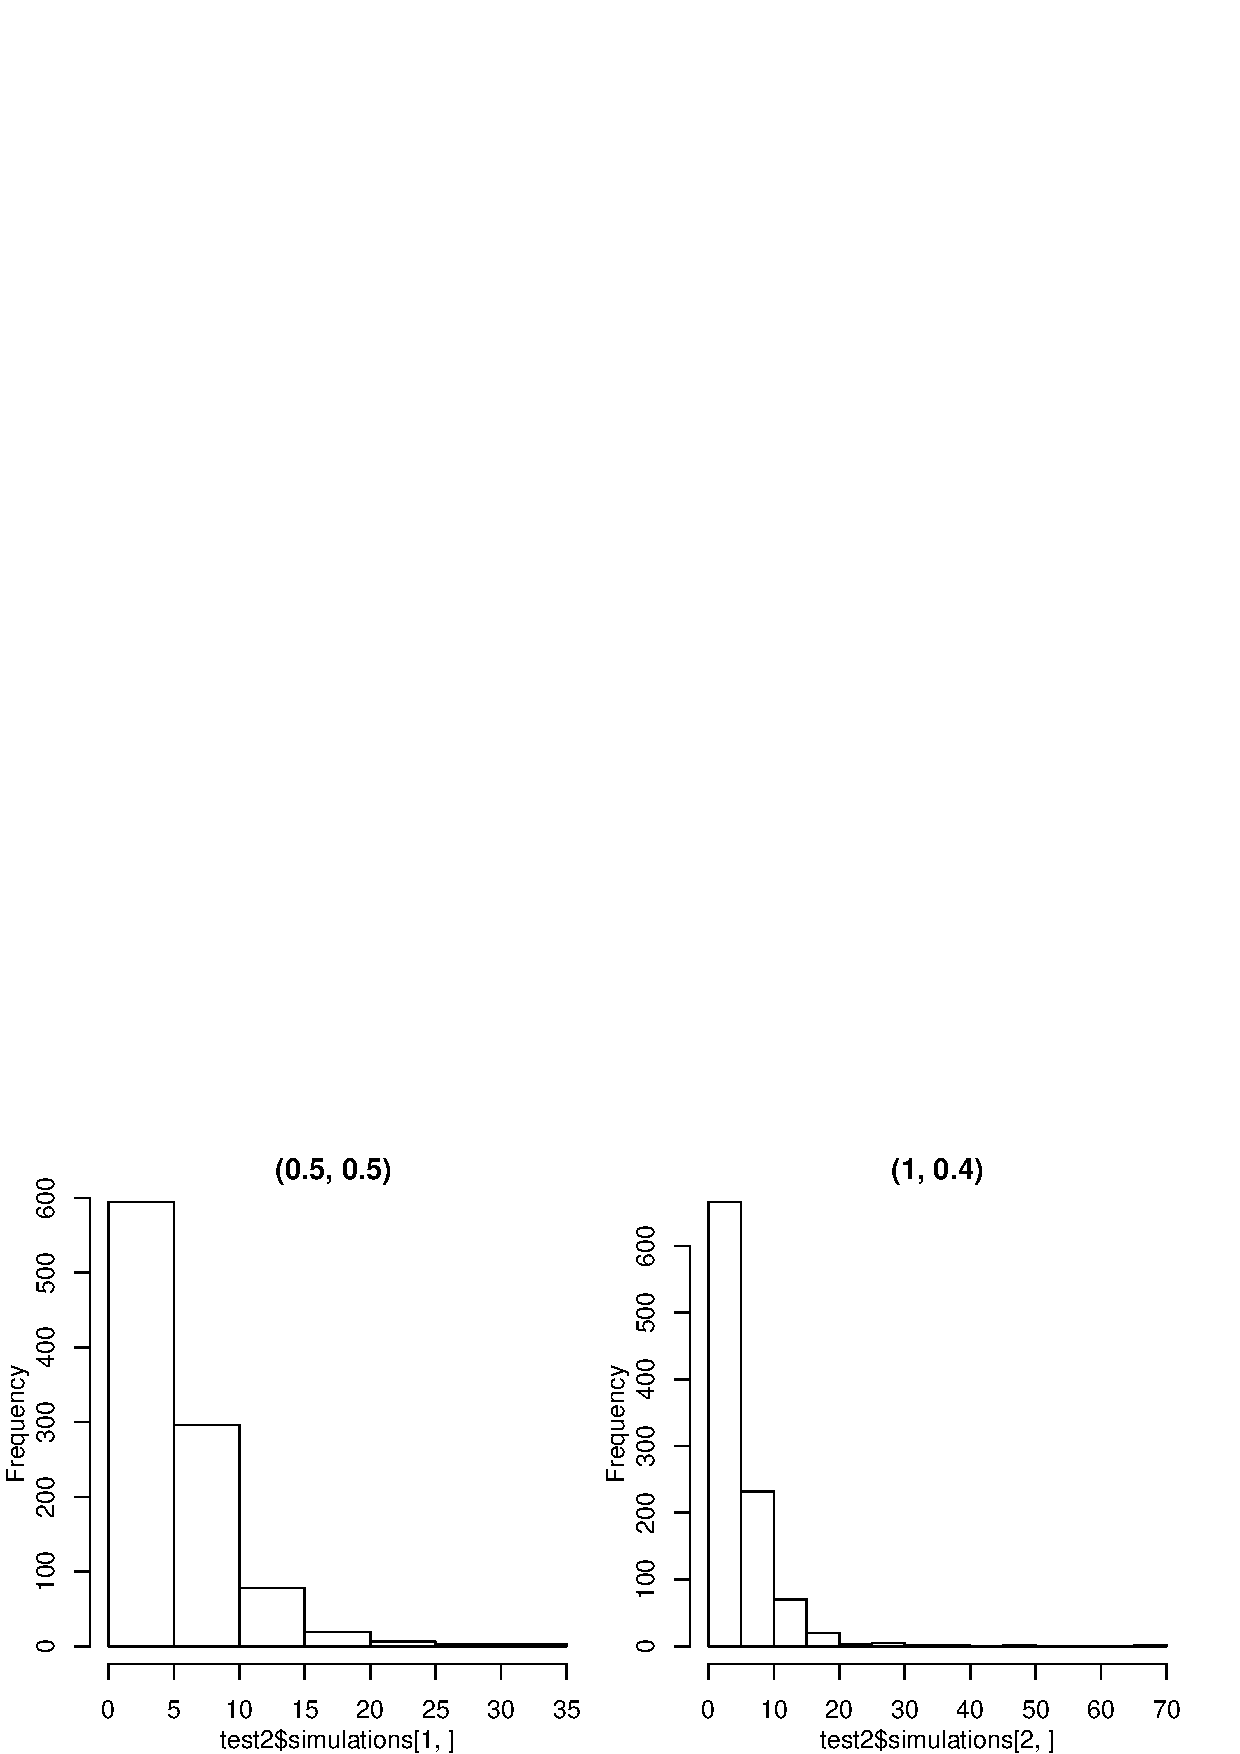
\includegraphics{geoRglmintro-009}
\label{fig:simulation}
\caption{Simulated data}
\end{figure}
Observe that the upper half of the figure corresponds to observation
times equal to 5, where the simulated counts are larger.


\paragraph*{Exercise}

Generate a simulation from a spatial binomial-logit model.


\section{MCMC SIMULATION}

The core part of \pkg{geoRglm} consist of generating MCMC simulations from
the conditional distibution of the random effects
at the data locations given the actual observed data. Such a simulation
algorithm 
is needed for any likelihood inference in generalised linear spatial
models (prediction, Bayesian inference and parameter estimation). Here
we consider the fixed parameter case, which is implemented in the
function \code{glsm.mcmc}.

The function uses a Langevin-Hastings MCMC algorithm for simulating from the conditional distribution.
The nugget effect parameter (microscale variation) in the underlying Gaussian field can be set to a fixed value. 
The same applies for the smoothness and anisotropy parameters. Options for taking covariates (trends) into 
account are also included.

An example for Poisson data where we assume a logarithmic link, and
where all parameters are fixed is shown below 
(for illustration purposes, some parameter values are just taken).  

First we need to tune the algorithm by scaling the proposal variance so that acceptance rate is approximately 60 percent (optimal
acceptance rate for Langevin-Hastings algorithm). This is done by trial and error. 
\begin{Schunk}
\begin{Sinput}
> model2 <- list(cov.pars = c(1, 1), beta = 1, family = "poisson")
> mcmc2.test <- mcmc.control(S.scale = 0.2, thin = 1)
> test2.tune <- glsm.mcmc(p50, model = model2, mcmc.input = mcmc2.test)
\end{Sinput}
\begin{Soutput}
iter. numb. 1000  : Acc.-rate =  0.877 
MCMC performed: n.iter. =  1000 ; thinning =  1 ; burn.in =  0 
\end{Soutput}
\end{Schunk}
After a few tryouts we decide to use \code{S.scale = 0.5}.
\begin{Schunk}
\begin{Sinput}
> mcmc2.tune <- mcmc.control(S.scale = 0.5, thin = 1)
> test2.tune <- glsm.mcmc(p50, model = model2, mcmc.input = mcmc2.tune)
\end{Sinput}
\begin{Soutput}
iter. numb. 1000  : Acc.-rate =  0.57 
MCMC performed: n.iter. =  1000 ; thinning =  1 ; burn.in =  0 
\end{Soutput}
\end{Schunk}
We also need to study convergence of the chain and how well the chain
is mixing. For this we use the functions in the \pkg{coda} package. We
first load \pkg{coda} and then create a \code{mcmc} object to
be used. Only a glimpse of the functionallity in \pkg{coda} is shown
here, we encourage the reader to investigate further.

\begin{Schunk}
\begin{Sinput}
> library(coda)
> test2.tune.c <- create.mcmc.coda(test2.tune, mcmc.input = mcmc2.tune)
\end{Sinput}
\end{Schunk}

We encourage the user to always make traceplots and autocorrelation
plots for all variables (in this case all 50 random effects). But in
order to not to clutter this introduction with a large number of
plots, we will present these plots for only one variable.

\newpage

\setkeys{Gin}{width=0.8\textwidth}
\begin{figure}[h!]
\centering
\begin{Schunk}
\begin{Sinput}
> test2.tune.c <- create.mcmc.coda(test2.tune$simulations[45, 
+     ], mcmc.input = list(S.scale = 0.5, thin = 1))
> par(mfrow = c(1, 2))
> plot(test2.tune.c, density = FALSE, ask = FALSE, auto.layout = FALSE)
> autocorr.plot(test2.tune.c, ask = FALSE, auto.layout = FALSE)
\end{Sinput}
\end{Schunk}
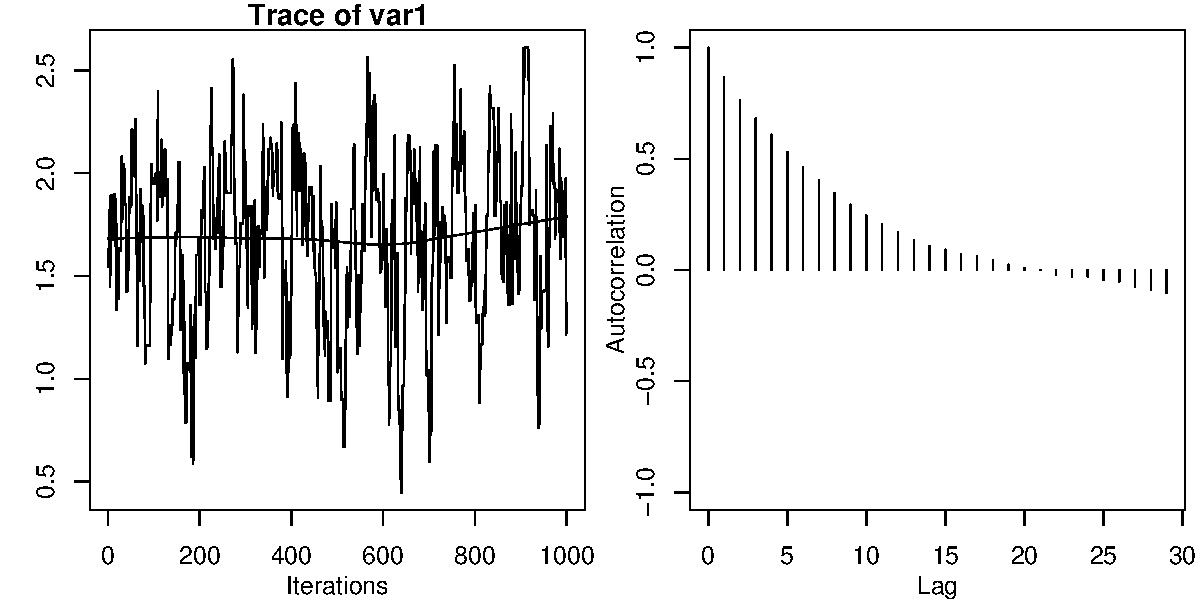
\includegraphics{geoRglmintro-013}
\label{fig:pois.krige}
\caption{Results from \texttt{glsm.mcmc} for one variable.}
\end{figure}

To reduce the autocorrelation of the samples we decide to subsample every 10 iterations (default); when working with larger data sets we may need to make a more 
extensive subsampling, say, storing only every 100 iterations.

\begin{Schunk}
\begin{Sinput}
> mcmc2 <- mcmc.control(S.scale = 0.5)
> test2 <- glsm.mcmc(p50, model = model2, mcmc.input = mcmc2)
\end{Sinput}
\begin{Soutput}
iter. numb. 1000  : Acc.-rate =  0.596 
iter. numb. 2000  : Acc.-rate =  0.607 
iter. numb. 3000  : Acc.-rate =  0.602 
iter. numb. 4000  : Acc.-rate =  0.61 
iter. numb. 5000  : Acc.-rate =  0.611 
iter. numb. 6000  : Acc.-rate =  0.595 
iter. numb. 7000  : Acc.-rate =  0.611 
iter. numb. 8000  : Acc.-rate =  0.615 
iter. numb. 9000  : Acc.-rate =  0.61 
iter. numb. 10000  : Acc.-rate =  0.625 
MCMC performed: n.iter. =  10000 ; thinning =  10 ; burn.in =  0 
\end{Soutput}
\end{Schunk}

\paragraph*{Exercise} Produce traceplots and autocorrelation plots
using the \pkg{coda} functions above (where you probably want
to use default values of the arguments \code{ask} and \code{auto.layout}) for
the MCMC output contained in \code{test2}.  



\section{SPATIAL PREDICTION}

For the model and data above we now consider spatial prediction, assuming that parameters are fixed.
Full Bayesian prediction methods are also implemented and will be presented in
Section~5. 

For computational
reasons we consider prediction at only two locations here.
Minimal mean square error prediction of the intensity at the two
locations (0.5, 0.5) and (1, 0.4). Here we use the object
\command{test2} created in
the previous section
\begin{Schunk}
\begin{Sinput}
> out2 <- output.glm.control(sim.predict = TRUE)
> pred.test2 <- glsm.krige(test2, locations = cbind(c(0.5, 
+     0.5), c(1, 0.4)), output = out2)
\end{Sinput}
\begin{Soutput}
 glsm.krige: Prediction for a generalised linear spatial model 
\end{Soutput}
\end{Schunk}

The output is a list including the predicted values (\code{pred.test2\$predict}), the prediction variances 
(\code{pred.test2\$krige.var}) and the estimated Monte Carlo standard errors on the predicted values (\code{pred.test2\$mcmc.error}). 
Printing out the predicted values and the associated Monte Carlo standard errors:
\begin{Schunk}
\begin{Sinput}
> cbind(pred.test2$predict, pred.test2$mcmc.error)
\end{Sinput}
\begin{Soutput}
         [,1]       [,2]
[1,] 5.503865 0.04906689
[2,] 4.934100 0.04225835
\end{Soutput}
\end{Schunk}
we see that the Monte Carlo standard errors (the errors due to the MCMC-simulation) are small 
compared to predicted values, which is very satisfactory.

By specifying \code{sim.predict = TRUE}, simulations are drawn from the predictive intensity at the two prediction locations (\code{pred.test2\$simulations}). 
These simulations are plotted in Figure~3. 
\setkeys{Gin}{width=0.8\textwidth}
\begin{figure}[h!]
\centering
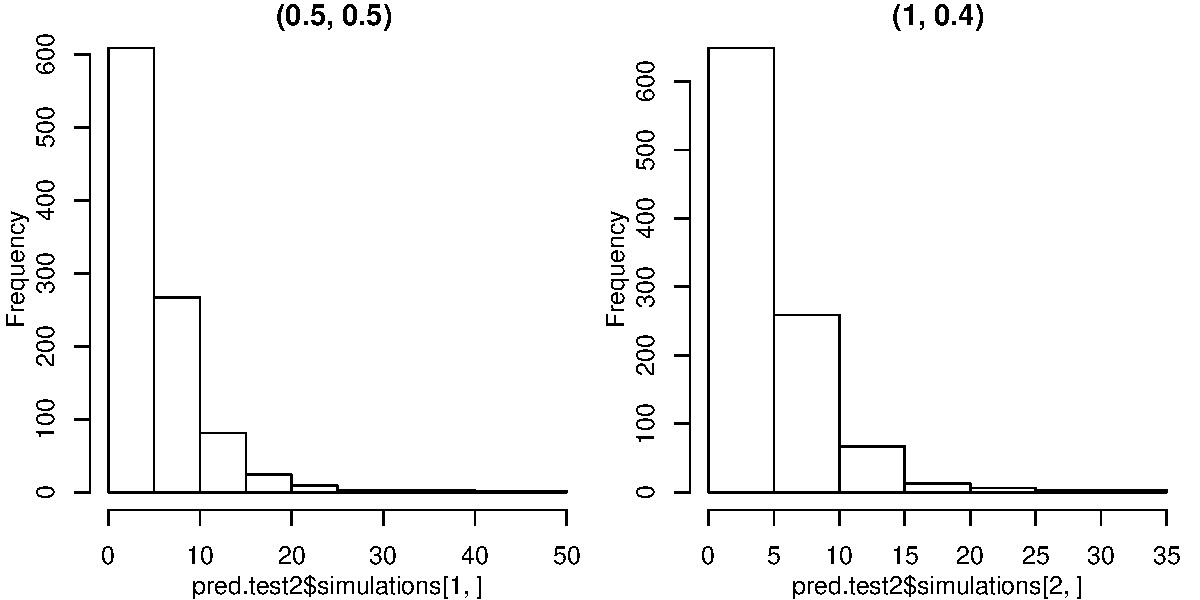
\includegraphics{geoRglmintro-017}
\label{fig:hist.sim.pk}
\caption{Histograms for simulations from the predictive distribution
for two locations.}
\end{figure} 

\paragraph*{Exercise}
Make prediction on a 40 by 40 regular grid, and afterwards visualise
predictions using the \pkg{geoR} function \code{image}. We suggest
to consult the section about prediction in the \pkg{geoR} introduction before starting.

\paragraph*{Exercise}
Binomial data can be specified by
\code{family="binomial"} in \code{glsm.mcmc}. The exercise consist in
repeating the commands above for the binomial data set \code{b50}.

\paragraph*{Remark}
In the classical Gaussian model there exist different kriging
flavours : simple kriging, ordinary kriging, etc. The prediction above
for a GLSM corresponds to simple kriging because all parameters are
fixed. Ordinary and Universal kriging in the Gaussian model
corresponds to using a uniform flat prior on the beta parameter. For a
GLSM, the corresponding prediction method is not implemented in the
functions above. However, a uniform flat prior on $\beta$ parameter is
considered in the next section on Bayesian inference, and in addition
it is also
implemented for fixed covariance parameters in the two functions \code{pois.krige} and \code{binom.krige}. 



\section{BAYESIAN ANALYSIS}

Bayesian analysis for the Poisson-log normal model and the binomial-logit model is implemented by the functions 
\command{pois.krige.bayes} and \command{binom.krige.bayes}, respectively.
Model parameters can be treated as fixed or random.        

As an example consider first a model without nugget and including uncertainty in the $\beta$ and $\sigma^2$ parameters (mean and variance of the random effects $S$, respectively). 
A Bayesian analysis is made by typing commands like: 
\begin{Schunk}
\begin{Sinput}
> prior5 <- prior.glm.control(phi.prior = "fixed", phi = 0.1)
> mcmc5.tune <- mcmc.control(S.scale = 0.01, thin = 1)
> test5.tune <- pois.krige.bayes(p50, prior = prior5, mcmc.input = mcmc5.tune)
\end{Sinput}
\begin{Soutput}
pois.krige.bayes: model with mean being constant
iter. numb. 1000 ; Acc.-rate = 0.98 
MCMC performed: n.iter. =  1000 ; thinning =  1 ; burn.in =  0 
Only Bayesian estimation of model parameters 
\end{Soutput}
\end{Schunk}

Now chose \code{S.scale} (Acc-rate=0.60 is preferable).  
After having adjusted the parameters for the MCMC algorithm and
checking the output we run an analysis (where we here omit the
printing of the messages from the MCMC iterations for brevity).
\begin{Schunk}
\begin{Sinput}
> mcmc5 <- mcmc.control(S.scale = 0.075, thin = 100)
> out5 <- output.glm.control(threshold = 10, quantile = c(0.05, 
+     0.99))
> test5 <- pois.krige.bayes(p50, locations = t(cbind(c(2.5, 
+     3), c(-6050, -3270))), prior = prior5, mcmc.input = mcmc5, 
+     output = out5)
\end{Sinput}
\end{Schunk}

The output is a list which contains the five arguments \code{posterior}, \code{predictive}, \code{model}, \code{prior} and \code{mcmc.input}. 
The \code{posterior} contains information
on the posterior distribution of the parameters, and the conditional simulations of the signal 
$g^{-1}(S)$ at the data locations. 
The \code{predictive} contains information on the predictions, where 
\code{predictive\$median} is the predicted signal and \code{predictive\$uncertainty} is the associated uncertainty.
The \code{threshold = 10} argument gives probabilities of the predictive distribution of the signal being less 
than 10 (\code{test5\$predictive\$probability}).
The \code{quantiles = c(0.05,0.99)} gives the 0.05 and 0.99 quantiles of the predictive distribution of the signal 
(\code{test5\$predictive\$quantiles}).

Below we show the simulations from the posterior distribution of the signal at a few data locations.
\setkeys{Gin}{width=\textwidth}
\begin{figure}[h!]
\centering
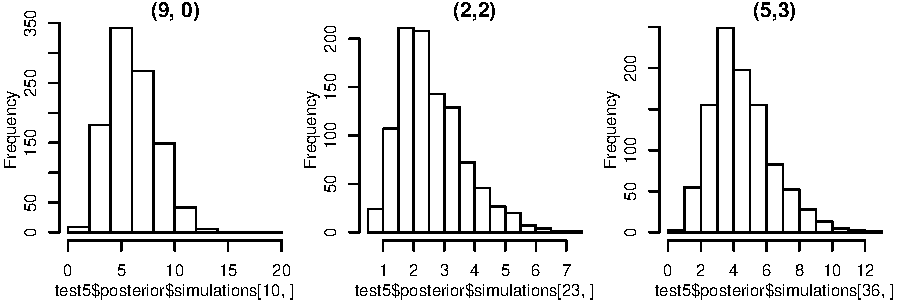
\includegraphics{geoRglmintro-021}
\label{fig:hist.sim.bayes}
\caption{Histograms}
\end{figure}

Now we consider an example with a random correlation scale parameter phi and a positive nugget for the random effects S. The program is using a discretised prior for phi, where the discretisation is given by
the argument \code{phi.discrete}). The argument \code{tausq.rel = 0.05} gives the relative nugget for S, i.e. the relative 
microscale variation.
\begin{Schunk}
\begin{Sinput}
> mcmc6.tune <- mcmc.control(S.scale = 0.075, n.iter = 2000, 
+     thin = 100, phi.scale = 0.01)
> prior6 <- prior.glm.control(phi.prior = "uniform", phi.discrete = seq(0.02, 
+     1, 0.02), tausq.rel = 0.05)
> test6.tune <- pois.krige.bayes(p50, prior = prior6, mcmc.input = mcmc6.tune)
\end{Sinput}
\end{Schunk}

Acc-rate=0.60 , acc-rate-phi = 0.25-0.30  are preferable. 
After having adjusted the parameters for the MCMC algorithm and checking the output we run an analysis.\\
\strong{WARNING: RUNNING THE NEXT COMMAND CAN BE TIME-CONSUMING}
\begin{Schunk}
\begin{Sinput}
> mcmc6 <- mcmc.control(S.scale = 0.075, n.iter = 4e+05, 
+     thin = 200, burn.in = 5000, phi.scale = 0.12, phi.start = 0.5)
> test6 <- pois.krige.bayes(p50, locations = t(cbind(c(2.5, 
+     3.5), c(-60, -37))), prior = prior6, mcmc.input = mcmc6)
\end{Sinput}
\end{Schunk}

Below we show the posterior distribution of the two covariance parameters and the beta parameter.
\setkeys{Gin}{width=\textwidth}
\begin{figure}[h!]
\centering
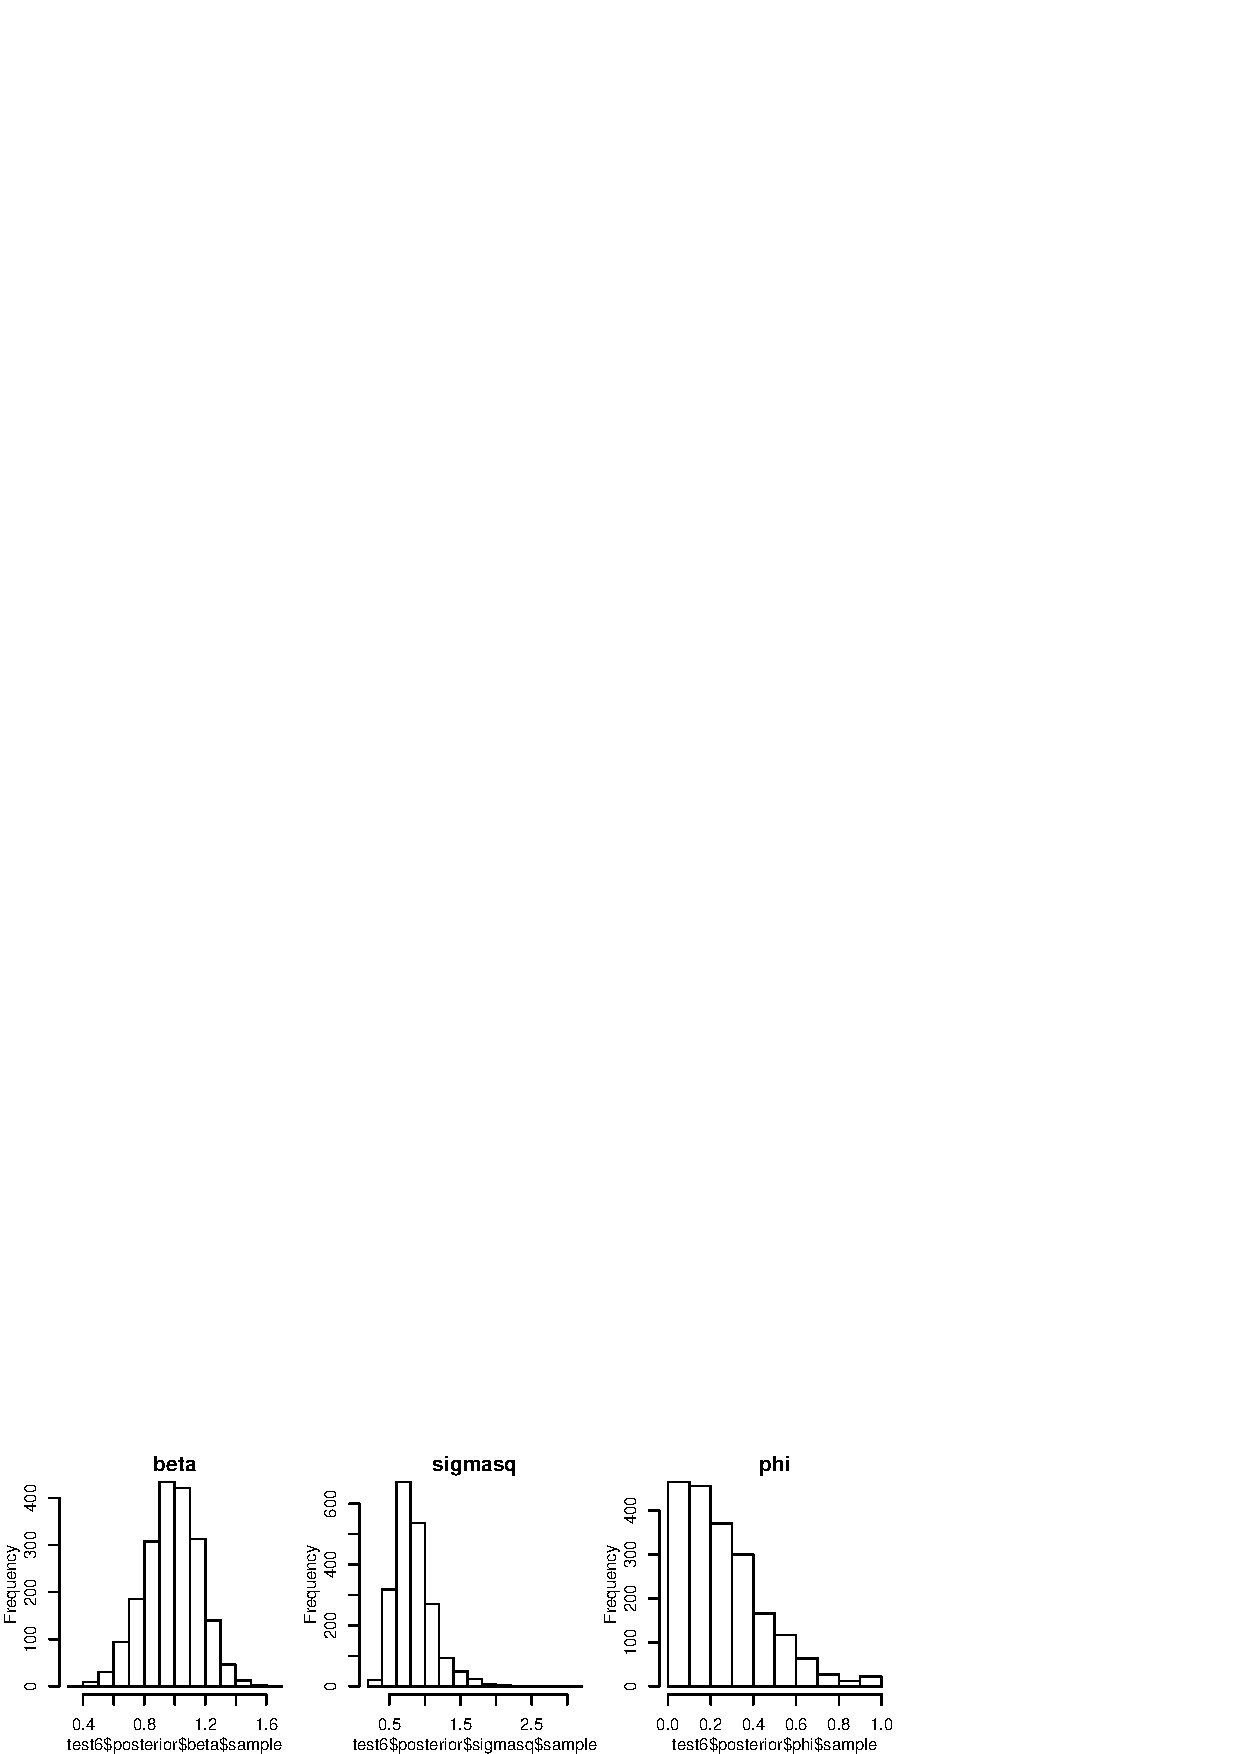
\includegraphics{geoRglmintro-024}
\label{fig:posterior}
\caption{Samples from the posterior}
\end{figure}


\paragraph*{Exercise}	
Use \pkg{coda} and the function \code{create.mcmc.coda} to investigate
the convergence and mixing of the MCMC algorithm for the examples above. 


\paragraph*{Exercise}
Construct similar commands as above using the function \command{binom.krige.bayes} on the data set \code{b50} yourself. 


\paragraph*{Remark}
The Bayesian inferential functions differ from the functions used in
the fixed parameter case in the following two ways : A. there exist two
functions, one for binomial data and for Poisson data. B. the Bayesian inferential procedure has not been
split into two functions, a MCMC function and prediction function,
similar to \code{glsm.mcmc} and \code{glsm.krige}. The main reason for
these differences is historical, the functions \code{glsm.mcmc} and
\code{glsm.krige} were introduced in geoRglm version 0.8-0 in the
spring 2004. A reason for not restructuring the Bayesian functions
similarly has been compatibility with the \pkg{geoR}
function \code{krige.bayes} (in addition to the lack of
time for doing so !).


\section{ADDITIONAL INFORMATION }  

Package \pkg{geoRglm} also contain some functions for likelihood inference
(MCMC-MLE). They are relatively slow to use, and have therefore not
been included in this introduction. 

We strongly encourage the user to study the relevant literature and
also the \pkg{geoRglm} homepage before starting using the package.


\end{document}
